\section{Abwägung des Einsatzes eines Informationsmanagers an der Hochschule Emden/Leer - JL}
\label{section_einsatz_cio}
\textit{Autor: Julia Lübke}

Das Soll-Konzept analysiert die Ist-Situation um den derweilen Zustand der  Hochschule Emden/Leer zu ermitteln. Daraus lässt sich erkennen, ob es generell einer Verbesserung des Informationsmanagements in der Zukunft bedarf und wo diese anzusetzen sind oder ob noch kein Informationsmanagement besteht und aufgebaut werden muss. Dazu sind verschiedene Aspekte zu beleuchten. Neben der Anforderung des zukünftigen Marketings, den technischen Neuerungen und der darauf folgenden Umsetzung ist zu klären, ob die Hochschule Emden/Leer eine Führung im Bereich des strategischen und operativen Informationsmanagements benötigt.

Im klassischen Informationsmanagement ist dies die Aufgabe eines Informationsmanager, dem sogenannten Chief Information Officer. Wie auf der Abbildung \ref{fig_def_inm} zu erkennen, arbeitet der Informationsmanager dabei als zentrale Schnittstelle zwischen technischen, organisatorischen und wirtschaftlichen Teilbereichen und dient dort als sogenannter Mittler zwischen den verschiedenen Bereichen und untersucht dabei die Informations- und Kommunikationstechniken in allen unterschiedlichen Bereichen um diese sinnvoll einzusetzen. 
\footcite[86]{definition_informationsmanager}

\begin{figure}[h!]
	\centering
	\includegraphics[width=10cm]{kapitel/gruppe3/bilder/definition_informationsmanager}
	\caption{Definition Informationsmanager}
	\label{fig_def_inm}
\end{figure}

\subsection{Analyse des Ist-Zustandes}
\label{subsection_analyse_ist_zustand}

Bezug nehmend auf das Organigramm aus Abbildung \ref{fig_organigramm_HS} der Hochschule Emden/Leer und der Bewertung aus  \ref{section_bewertung_gewichtung} ist festzuhalten, dass der Hochschule kein klassisches Informationsmanagement zugrunde liegt, sondern ein zentrales Informationssystem. Es werden bereits Informationen verwaltet und weitergegeben, jedoch nicht an zentraler Stelle. Zentrale Systeme, siehe Abbildung \ref{fig_zentrale_systeme}, Kapitel \ref{section_zustaendigkeiten}, sowie unterschiedliche Möglichkeiten werden für alle zur Verfügung gestellt und in Anspruch genommen. 

Es gibt keine Verwaltung, sondern verschiedene Bereiche, die unterteilt sind in Arbeitsgruppen, Abteilungen sowie Rechenstelle und Pressestelle. Weiterhin beinhaltet das Informationssystem verschiedene Prozesse zum Datenaustausch bzw. Datenfluss und Back-up-Transfer aus verschiedenen Systemen.  Die Nutzung des gegenwärtigen Informationssystems wird unterschiedlich stark genutzt oder ausgelastet. 

Von den zentralen Einrichtungen nehmen das Hochschulrechenzentrum und die Bibliothek einen wichtigen Platz in der Hochschule Emden/Leer ein. Das Hochschulrechenzentrum übernimmt derweil viele Aufgaben der Informationsverwaltung und Planung. Doch nicht nur da werden Informationen gesammelt und ausgewertet. Die Hochschule in Emden definiert eine ganze Reihe von Arbeitsgruppen, beispielsweise die Arbeitsgruppe Zahlen, Daten, Fakten, die Kennzahlen der Hochschule und der einzelnen Fachbereiche sammelt und diese auswertet und an gewünschte Stellen weitergibt.  

Aktuell besteht keine erweiterte Vernetzung unterschiedlicher Intranetzsysteme zwischen verschiedenen Hochschulen. Lediglich im Bereich der Bibliothek werden Inhalte an mehreren Standorten gemeinsam genutzt. Abschließend ist zu erwähnen, dass die Hochschule Emden/Leer auch keine Einzelperson oder ein Gremium als zentrale Informationsverwaltung nutzt.


\subsection{Betrachtung des zu erwartenden Soll-Zustandes }
\label{subsection_betrachtung_soll}

Nach Betrachtung der Best-Practice-Beispiele aus Kapitel \ref{chapter_best_practice_beispiele} lässt sich erkennen, dass jede Hochschule und auch Universität den Umgang des Informationsmanagements anders angeht. So spielen verschiedene Faktoren eine Rolle, die an jeder Hochschule/Universität unterschiedlich ausgelegt sind. Ein Vergleich der betrachteten Universitäten mit der Hochschule Emden/Leer zeigt, dass Emden eine wesentlich kleinere Institution ist und somit andere Ansprüche hat und weniger komplexe Strukturen besitzt, als beispielsweise die WWU Münster, die über 40.000 Studierende pflegt. 

Trotz unterschiedlich integrierter Möglichkeiten der unterschiedlichen Universitäten zur Umsetzung des jeweiligen Informationsmanagements gibt es doch Bereiche, die gleich oder zumindest ähnlich sind. So sind Bibliotheken, Gremien, Ausschüsse, ebenso wie Fachbereiche, das Rechenzentrum und auch das Präsidium Teil einer jeden Hochschule oder Universität. 

Es ist also zu schauen, wo sich das Informationsmanagement als zentrale Informationsquelle ansetzen lässt, um mehrere Bereiche und Bestandteile untereinander zu verbinden. Fakt ist, dass es in Emden bereits drei Arbeitsgruppen gibt, die bestimmte Informationen gewinnen und filtern.  So wäre zu betrachten, wie die Zentralisierung einer übergeordneten Informationsquelle und -weitergabe zu bewerkstelligen wäre und wie der Aufbau einer neuen Struktur die Möglichkeit zur Verbesserung des Informationsaustausches aussehen könnte. 

In Kapitel \ref{subsection_zentralisierung_integration} wird beschrieben, dass die meisten Hochschulen und Universitäten unter einer neu geschaffenen Organisation arbeiten. Dabei spielen das Rechenzentrum, die Bibliothek und die Verwaltung immer eine Rolle in einer solchen Organisation. Kein Konzept ist maßgeschneidert und nicht auf jede Hochschule oder Universität anwendbar.

\subsubsection{Empfehlungen der ZKI bezüglich des Informationsmanagers}
\label{subsubsection_zki}

Neben den verschiedenen Projekten und Einrichtungen, die im Kapitel \ref{chapter_best_practice_beispiele} beleuchtet werden, und aufzeigen, wie mit dem Informationsmanagement umgegangen wird, gibt es noch die Zentren für Kommunikation und Informationsverarbeitung (ZKI) in Lehre und Forschung, die Empfehlungen für Hochschulen bezüglich des Informationsmanagements und besonders Empfehlungen für den Informationsmanager aussprechen.

Blickend auf die Publikation der ZKI basierend auf einer Studie der CIOs und IT-Governance an deutschen Hochschulen aus dem Jahre 2014 wurden über mehrere Jahre von der Kommission für IT-Infrastruktur der Deutschen Forschungsgemeinschaft (KfR) hinweg folgende Empfehlungen für Hochschulen ausgesprochen.

Zwischen 2001 - 2005 gab die KfR folgende Empfehlung:

\textit{" Aufgrund der Relevanz der Informationsverarbeitung für alle Bereiche der  Hochschule wird empfohlen, 
	einen Generalverantwortlichen für Information und  Kommunikation (CIO, Chief Information Officer) 
	in der Hochschulleitung oder ein geeignetes Leitungsgremium mit entsprechenden 
	Entscheidungskompetenzen mit der Entwicklung und  Koordinierung aller IuK-Aufgaben 
	zu betrauen."}\footcite[3]{zki_studie_cio_2014}

Zwischen 2006 - 2010 werden weitere Ausführungen genannt:

\textit{" Integriertes Informationsmanagement ist daher zur wesentlichen Aufgabe bei der Planung des 
	Einsatzes moderner Techniken von Information und Kommunikation für die Hochschulen geworden. 
	Eine solche Planung setzt die Position eines Verantwortlichen für Information und Kommunikation 
	als Mitglied der Hochschulleitung (CIO: Chief Information Officer) voraus, wie er in der Wirtschaft 
	und an verschiedenen Hochschulen bereits etabliert ist."}\footcite[16]{zki_studie_cio_2014}

Die KfR Empfehlungen zwischen 2011-2015 werden noch weiter ausgebaut:

\textit{"In der Hochschulpraxis lassen sich vier unterschiedliche Umsetzungstypen beobachten:  Strategischer CIO mit Leitungsfunktion: Ein Vizepräsident - oder eine Vizepräsidentin - ist explizit für das Informationsmanagement zuständig. Teilweise übernimmt auch der Kanzler die Zuständigkeit für das Informationsmanagement.}

\begin{itemize}
	\item \textit{Strategischer CIO mit Stabsfunktion: Ein Hochschullehrer oder IT-Manager - 
		bzw. Hochschullehrerin/IT-Managerin - im Präsidialstab koordiniert das Informationsmanagement.} 
	\item \textit{Operativer CIO: Der Leiter - bzw. die Leiterin - einer zentralen 
		Informationsinfrastruktureinrichtung fungiert gleichzeitig als CIO der Hochschule.}
	\item \textit{Kollektiver CIO: Die CIO-Funktion wird von einem Lenkungsausschuss mit zwei bis 
		drei Personen ausgeübt, der allerdings - anders als die traditionelle Senatskommission - über 
		unmittelbare Entscheidungsbefugnisse verfügt.}
\end{itemize}
\textit{Jede dieser CIO-Umsetzungsvarianten hat ihre Vor- und Nachteile. Es hängt von den 
	Gegebenheiten an den Hochschulen und insbesondere auch von Personen ab, welche 
	Umsetzung die am besten geeignete ist. Wichtig ist, dass der CIO - in welcher Form 
	auch immer - einen unmittelbaren Zugang zur Hochschulleitung hat und die IT-Belange 
	der gesamten Hochschule strategisch - mit unmittelbarer Richtlinien- und 
	Entscheidungskompetenz - fährt und verantwortet."} \footcite[17]{zki_studie_cio_2014}

Abschließend ist zu sagen, dass die ZKI/KfR einer Hochschule eine zentrale Informationsschnittstelle in Form eines CIOs oder eines CIO-Gremiums empfiehlt.

\subsubsection{Informationsmanager oder Gremium als zentrale Informationsschnittstelle}
\label{subsubsection_cio_gremium}

Der Aufbau eines Informationsmanagements bedarf vieler Schritte und Überlegungen (siehe Abschnitt \ref{begriffsdefintion_inm}). Neben den Veränderungen und deren Umsetzung ist zu klären, ob der bisherige Austausch der Informationen der Hochschule Emden/Leer durch eine zentrale Einrichtung oder einer Einzelperson und entsprechenden Verantwortlichkeiten geregelt werden soll. Um dies in ein reales Szenario zu bekommen, sind die Möglichkeiten aufzuzeigen und ein entsprechend passendes Modell für die Hochschule Emden/Leer zu entwickeln. Dazu werden in Abschnitt  \ref{section_betr_hochschule}, ebenso wie in der Studie der ZKI verschiedene Konzepte des Chief Information Officers (CIO) aufgezeigt. 

Ein einheitliches Konzept ist nicht gegeben, sodass nicht jede Lösung auch passend für die Hochschule Emden/Leer ist. Die betrachteten Universitäten haben ein anderes Anforderungsprofil an ein Informationsmanagement und deren zentrale Leitung als Emden, die wesentlich kleinere und weniger komplexe Strukturen besitzt. Zu den betrachteten Best-Practice-Beispielen lassen sich zusätzlich die Empfehlungen der KfR heranziehen. 

Alle haben gemeinsam, dass das Verwalten der Informationen aus einer Schnittstelle heraus geschieht. Auch dieses Konzept ist für die Hochschule Emden/Leer zu überlegen. Nun stellt sich die Frage, wo diese Schnittstelle anzusetzen ist und wer die Aufgaben übernehmen soll. Verschiedene Möglichkeiten sind hier zu betrachten. Zum einen gibt es das Personenmodell, den CIO, beschrieben in \ref{anforderungsprofil_informationsmanager} und \ref{eingliederung_informationsmanager} der die Schnittstelle bildet, zum anderen gibt es die Möglichkeit eines CIO-Gremiums. 


\textbf{Personenmodell:\newline}
Eine Person wird als Informationsmanager herangezogen und übernimmt die in den Abschnitten \ref{aufgaben_funktionen_informationsmanager}, \ref{anforderungsprofil_informationsmanager} und \ref{eingliederung_informationsmanager} angegebenen Aufgaben, die hochschulangepasst sind. Dabei ist zu betrachten, wer diese Aufgabe übernehmen soll. Der CIO kann aus der Privatwirtschaft geordert werden. Dabei ist zu bedenken, dass dafür eine Menge Ressourcen benötigt werden. Neben dem aufwendigen Bewerbungsprozess und der Einstellung erfolgt die Einarbeitungszeit und die Einführung des Informationsmanagements durch den CIO. Als weiterer Punkt sind noch die erhöhten Personalkosten in dieser Zeit zu nennen.

Neben der Möglichkeit einen CIO aus der Privatwirtschaft zu holen, besteht auch die Möglichkeit einen hochschulinternen Mitarbeiter zu involvieren. Der Bewerbungszeitraum und die Einarbeitung verringern sich, da ein bestehender Mitarbeiter die Hierarchie und die Arbeitsweise der Hochschule Emden/Leer bereits versteht und kennt. Allerdings ist nicht zu verachten, dass diese Person, entweder eine Mehrbelastung durch die zusätzlichen Aufgaben des Informationsmanagers tragen muss oder für die vorherige Stelle ein neuer Mitarbeiter gesucht werden müsste, was auch in diesem Fall mit einem erhöhten Kosten- und Zeitaufwand verbunden wäre.


\textbf{Gremiummodell:\newline }
Soll das Informationsmanagement allerdings nicht nur von einer einzelnen Person betrieben werden, ist zu klären, wer diese Aufgabe übernehmen soll. Dazu ist immer in Vergleich zu setzen, welche Parameter greifen. Die Studie der ZKI besagt, Bezug nehmend auf die Abbildung \ref{fig_herkunft_cio_hochschulen}, dass die Gremienmitglieder aus ganz unterschiedlichen Bereichen der Hochschule kommen. Ist dies der Fall und ein Gremium wird ernannt, ist ein Arbeitsaufwand der anfallenden CIO Tätigkeiten auf alle Mitglieder aufgeteilt. So ist der Gesamtaufwand pro Person prozentual geringer als bei einer einzelnen Person, die mindestens 50\% ihrer Zeit in CIO-Aufgaben investiert. 



\begin{figure}[h!]
	\centering
	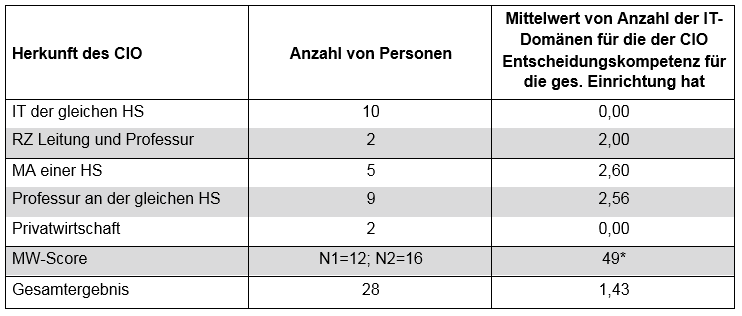
\includegraphics[width=\textwidth]
	{kapitel/gruppe3/bilder/herkunft_cio_hochschulen}
	\caption{Herkunft des CIO an verschiedenen Hochschulen, nach ZKI CIO-Studie}
	\label{fig_herkunft_cio_hochschulen}\footnote{\cite[8]{zki_studie_cio_2014}}
\end{figure}



\subsection{Empfehlung für die Hochschule Emden/Leer}
\label{empfehlung_cio}

Durch stetig wachsende Anforderungen besonders im Bereich der technischen Neuerungen und deren Umsetzung sowie Weitergabe und Verarbeitung von Informationen spricht die KfR seit Jahren Empfehlungen bezüglich eines Informationsmanagers an Hochschulen aus. Durch zusätzliches Betrachten der Best-Practice-Beispiele wird gezeigt, dass jede Hochschule andere Anforderungen besitzt und bezüglich ihrer Größe, Lage und Ansprüche anders mit einem Informationsmanagement umgeht, jedoch alle gemeinsam haben, dass eine zentrale Schnittstelle gebildet wird, die zusammenlaufende Informationen verarbeitet, auswertet und weitergibt.

Nicht jede Lösung eignet sich dabei für jede Hochschule. In einer Studie der ZKI geht dies ebenfalls hervor. Die Studie befasst sich mit dem Informationsmanager und spricht dabei Empfehlungen für Hochschulen aus. Dabei ist festzuhalten, dass es neben dem Einzelpersonen-Modell auch ein CIO-Gremium-Model geben kann, je nach Bedürfnis der Hochschule. Eine Einzelperson kann hierbei vorteilhafter sein als ein Gremium, dennoch ist zu betrachten, dass ein enormer personeller Kosten- und Zeitfaktor entstehen wird, da nicht zu verachten ist, dass das Aufbauen einer solchen Struktur Jahre in Anspruch nimmt. Es ist daher abzuwägen, ob sich dieser finanzielle Aufwand für die Hochschule Emden/Leer lohnt.

Da Emden bereits die drei Arbeitsgruppen Zahlen, Daten und Fakten, Web und Moodle besitzt, detaillierter beschrieben in \ref{subsection_arbeitsgruppen_informationsaustausch}, die wichtige Informationen sammeln und verarbeiten, wäre der Hochschule Emden/Leer eine Empfehlung zu einem CIO-Gremium auszusprechen. Durch die bereits existierenden Arbeitsgruppen ist aus jedem Bereich bereits ein Vertreter vorhanden. 

Die Hochschule Emden/Leer ist diesbezüglich schon gut aufgestellt, um weitere Schritte beim Einführen dieses Konzeptes einleiten zu können. Die anfallenden Aufgaben werden auf das gesamte Gremium aufgeteilt, sodass eine geringere Mehrbelastung entsteht. Abb. \ref{fig_moegliches_gremium} zeigt die Umstellung des Organigramms der Hochschule Emden/Leer, als mögliche Organisation. Das Gremium unterliegt dabei der Hochschulleitung. Da das Rechenzentrum bereits wichtige und zentrale Aufgaben besonders im technischen Bereich übernimmt, wäre es sinnvoll das Gremium aus dem Bereich heraus zu gründen. 

\begin{figure}[h!]
	\centering
	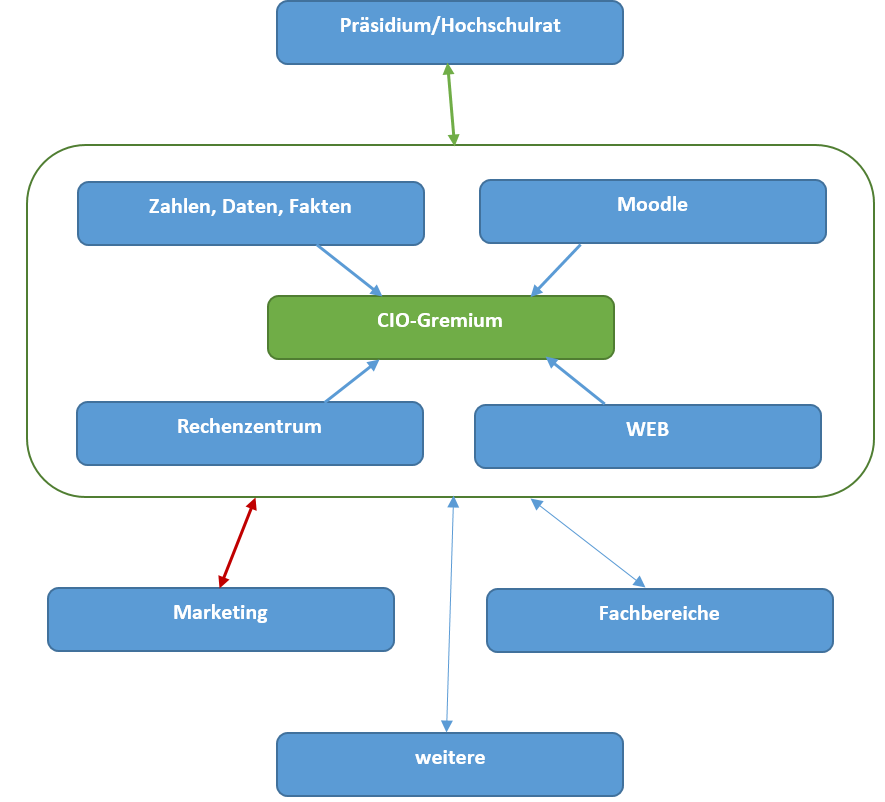
\includegraphics[width=\textwidth]
	{kapitel/gruppe3/bilder/moegliches_cio_gremium}
	\caption{Umstellung/Änderung des Organigramms der Hochschule Emden 	hinsichtlich eines CIO Gremiums}	
	\label{fig_moegliches_gremium}
\end{figure}

In Verbindung mit den drei bereits existierenden Arbeitsgruppen würde sich eine Mischform zwischen strategischem und kollektivem CIO für die Hochschule Emden/Leer anbieten. Das bietet die Möglichkeit sich den Gegebenheiten der Hochschule anzupassen und ein auf Emden/Leer wäre, dass das CIO-Gremium eng mit dem Marketing zusammenarbeitet und somit von der vorgestellten Möglichkeit Feedback zu sammeln, beschrieben in \ref{feedback} profitieren würde. So können anfallende Probleme direkt diskutiert und Lösungen gefunden werden. 


